\documentclass[a4paper,12pt]{article}
	\usepackage{graphicx}
	\usepackage[utf8]{inputenc}
	\usepackage[T1]{fontenc}
	\usepackage{listings}
	\usepackage{color}
	\usepackage{amsmath}

	\definecolor{dkgreen}{rgb}{0,0.6,0}
	\definecolor{gray}{rgb}{0.5,0.5,0.5}
	\definecolor{mauve}{rgb}{0.58,0,0.82}

	\lstset{frame=tb,
	  language=Python,
	  aboveskip=3mm,
	  belowskip=3mm,
	  showstringspaces=false,
	  columns=flexible,
	  basicstyle={\small\ttfamily},
	  numbers=none,
	  numberstyle=\tiny\color{gray},
	  keywordstyle=\color{blue},
	  commentstyle=\color{dkgreen},
	  stringstyle=\color{mauve},
	  breaklines=true,
	  breakatwhitespace=true
	  tabsize=3
	}
	\title{ Mecânica Clássica I}
	\author{\small André Del Bianco Giuffrida\\ \small IFSC - USP\\ \small andre.giuffrida@usp.br}
	\date{}
\begin{document}
\maketitle
	Para um barco de massa m e velocidade inicial Vo, onde atua a força:
		\[ F(t)= -b e^{\alpha V(t)}\]
		
		\begin{figure}[h]
			\centering
			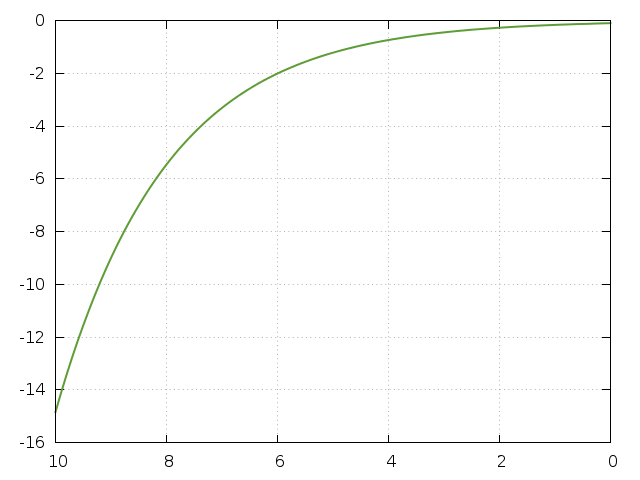
\includegraphics[scale=0.6]{3o0.png}
			\caption{$F(v)$ é no sentido contrário ao movimento}
		\end{figure}
		
	Podemos calcular $V(t)$ e também $x(t)$ do seguinte modo:
	
		\[ m \frac{dv}{dt} = -b e^{\alpha v} \to  m dv = -b e^{\alpha v} dt\]
		
		juntando as variáveis comuns
		
		\[ e^{-\alpha v} dv = \frac{-b}{m}  dt \] \[ \int_{v_0}^{v(t)} e^{-\alpha v} dv = \int_0^t \frac{-b}{m}  dt'\]
		\[ -\frac{1}{\alpha} e^{-\alpha v} \Bigg|_{v_0}^{v(t)}= \frac{-b}{m} t \]
		\[ e^{-\alpha v(t)} - e^{-\alpha v_0}= \frac{b \alpha}{m} t \]
		\[ v(t) = -\frac{ln(\frac{b \alpha}{m} t + e^{-\alpha v_0} ) }{\alpha } \]
		
		Aqui podemos obter o tempo de translado $t_t$ que demora para o barco atingir a velocidade $v(t_t)=0$:
		
		\[ 1 - e^{-\alpha v_0}= \frac{b \alpha}{m} t_t \]
		\[  t_t =( 1 - e^{-\alpha v_0} )\frac{m}{b \alpha} \]
		
		Calculando numericamente através do código em Python:
		
		
		\begin{lstlisting}
		#EulerMethod.py#
		
		from math import *
		import sys

		##
		#	Metodo de Euler simples
		#	Entradas: Velocidade inicial do barco
		#			Resolucao para a derivada (dt)
		#
		#	Saidas: Exibe na tela o tempo e sua respectiva
		#			velocidade instantanea
		##
		def Euler(Vi, dt):
			
			#constantes#
			m=100
			b=1
			alpha=3
	
			#condicaoe iniciais
			v=Vi 
			t=0
			
			#Enquanto a Velocidade nao cair para 1 por cento da velocidade inicial
			#(Tentativa de reduzir tempo de processamento!)
			while v > Vi*0.01 :		
				#Marcador de tempo
				t = t+dt
				#Calculo da velocidade
				v = v -(b/m)*exp(alpha*v)*dt
				#Exibicao na tela
				print t,v
		
		#chamada da funcao
		Euler(1,0.001)
		\end{lstlisting}
		
		\begin{figure}[h]
			\centering
			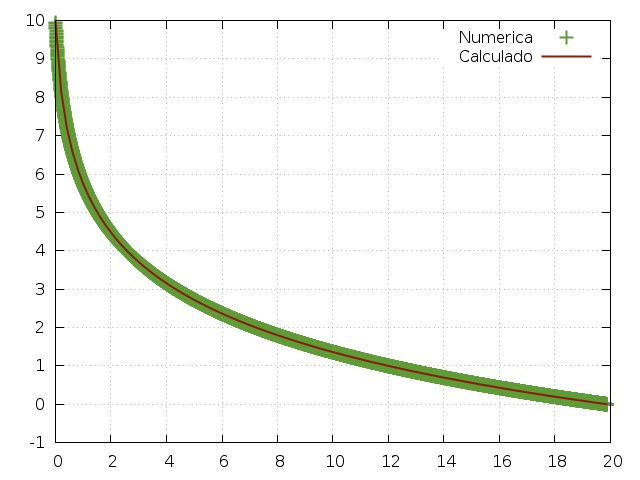
\includegraphics[scale=0.6]{3o1.png}
			\caption{$v(t)$ Numérica e Calculada}
		\end{figure}
		
		Já para obter-mos a posição em função do tempo temos:
		
		\[\frac{dx}{dt}=-\frac{ln(\frac{b \alpha}{m} t + e^{-\alpha v_0})}{\alpha}\]
		
		Integrando ambos os lados:
		
		\[\int_{x_0}^{x(t)}dx=\int_0^t-\frac{ln(\frac{b \alpha}{m}t'+e^{-\alpha v_0})}{\alpha}dt'\]
		
		\[ x(t) - x_0 = \int_0^t -\frac{ln(\frac{b \alpha}{m}t'+e^{-\alpha v_0})}{\alpha} dt' \]
		
		Para facilitar trocaremos $\frac{b \alpha }{m}$ por $A$ e $e^{-\alpha v_0}$ por B temos:
		
		\[ x(t)-x_0 = \frac{-1}{\alpha}\int_0^t ln(At' + B) dt'\]
		
		usando substituição de $At+B = u$ e depois aplicando integração por partes, temos:
		
		
		\[ x(t)-x_0 = \frac{-1}{\alpha} \Bigg[\frac{(At'+B)ln(At'+B)-At'}{A} \Bigg]_{0}^{t}\]
		\[ x(t)-x_0 = \frac{-1}{\alpha} \Bigg( \frac{(At+B)ln(At+B)-At}{A} -\frac{Bln(B)}{A} \Bigg)\]
		
		Agora voltando os valores para $A$ e $B$ obtemos a equação de $x(t)$
		
		\[ x(t) - x_0 = \frac{-1}{\alpha} \Bigg( \frac{(\frac{b\alpha}{m}t+e^{-\alpha v_0})ln(\frac{b\alpha}{m}t+e^{-\alpha v_0})-\frac{b\alpha}{m}t}{\frac{b \alpha}{m}} -\frac{e^{-\alpha v_0}ln(e^{-\alpha v_0})}{\frac{b\alpha}{m}} \Bigg) \]
		
		Simplificando fica:
		
		
		\[ x(t) = \frac{-m}{b\alpha^2}  \Bigg( \Bigg(\frac{b\alpha}{m}t + e^{-\alpha v_0}\Bigg)  ln\Bigg(\frac{b\alpha}{m}t + e^{-\alpha v_0}\Bigg) - \frac{b\alpha}{m}t +\alpha v_0e^{-\alpha v_0}\Bigg) + x_0 \]
		
		\begin{figure}[h]
			\centering
			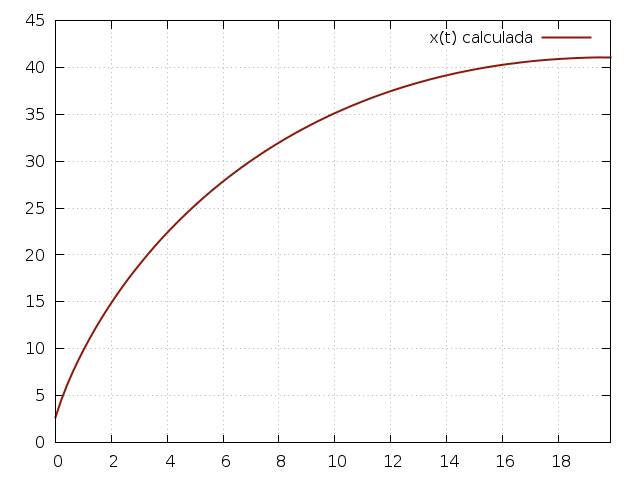
\includegraphics[scale=0.6]{3o2.png}
			\caption{$x(t)$ Calculada}
		\end{figure}	
	
	\paragraph \indent Observações: devido ao fato da modelagem ter sido feita em cima de uma força puramente dissipativa, podemos notar que não são quais quer valores de $\alpha$ e $b$ que resolvem o sistema, estes coeficientes têm de ser medidos por isso para plotar os gráficos foram usados os valores que mais se aproximavam do resultado esperado, a fim de modelar o problema e buscar uma estimativa de ordem de grandeza para estes valores.\\
	\indent Para todos os gráficos mostrados foram utilizados os seguintes valores: \\ 
	 $m=1 $ \\ 
	 \indent $b=0.1$ \\
	 \indent $\alpha=0.5$ \\
	 \indent  $V_0 = 10$ \\
	 
	
	
	\end{document}
	
